% =============================================================================
% Section: 06-business-value-metrics.tex | Rubric: Valor esperado
% Purpose: KPI principal y métricas del piloto; sin cifras inventadas.
% Style: es-CO académico-profesional, sin sobrepromesas; clasificar claims como
%        implementado/demo/pendiente; labels fig:/tab: estables (snake_case).
% =============================================================================
\section{Valor esperado y métricas}

El KPI principal es la \textbf{conversión de consulta por WhatsApp a pedido confirmado}. Esta métrica conecta el agente con valor de negocio sin caer en una promesa simplista de reducción de personal. Un piloto bien diseñado debe medir el antes y el después, porque hoy el proceso manual no necesariamente tiene línea base. Por eso la primera fase del piloto debe registrar tiempos, conversiones y fallbacks antes de declarar beneficios.

\begin{table}[htbp]
\centering
\caption{Métricas propuestas para el piloto controlado}%
\label{tab:metricas}
\small
\begin{tabular}{@{}>{\raggedright\arraybackslash}p{4cm}>{\raggedright\arraybackslash}p{6.2cm}>{\raggedright\arraybackslash}p{4cm}@{}}
\toprule
\textbf{Métrica} & \textbf{Qué muestra} & \textbf{Uso ejecutivo} \\ \midrule
Conversión a pedido confirmado & Porcentaje de consultas que terminan en pedido validado & KPI principal de valor. \\
Tiempo a confirmación & Minutos entre primer mensaje y resumen confirmado & Evalúa velocidad y fricción. \\
Pedidos incompletos & Casos que llegan a operación con datos faltantes & Mide calidad de captura. \\
Mensajes de aclaración & Número de preguntas necesarias por pedido & Mide eficiencia conversacional. \\
Fallback o escalamiento & Casos que el agente no debe resolver solo & Mide riesgo y carga humana. \\
Errores y reproceso & Pedidos corregidos o retenidos antes de producción & Mide daño operativo evitado. \\ \bottomrule
\end{tabular}
\end{table}

\subsection{Evidencia empírica externa para el piloto}

Tres estudios ayudan a ubicar el valor esperado de DeliverAI en una discusión empírica y no solo aspiracional. Brynjolfsson, Li y Raymond reportan, en un despliegue real con 5.172 agentes de soporte, que la asistencia conversacional basada en IA aumentó la productividad en 15\%, con mayor efecto en trabajadores novatos o de menor desempeño~\cite{brynjolfsson2025}. En un caso más cercano a una microempresa de comercio electrónico, Marcineková, Janáková Sujová y Ďurica encontraron que un chatbot atendió en promedio 74.2\% de las consultas, redujo el tiempo promedio de respuesta de 118.25 a 64 minutos y elevó la satisfacción de 3.73 a 4.27~\cite{marcinekova2025}. Como referencia de automatización transaccional a escala, Lacity, Willcocks y Craig documentaron en Telefónica O2 un piloto RPA completado en dos semanas, una capacidad interna casi independiente en 12 semanas y un caso de negocio con retorno de 10 a 12 meses para procesos seleccionados~\cite{lacity2015}.

La lectura para DeliverAI es deliberadamente conservadora: estos porcentajes no se trasladan mecánicamente al proyecto, porque los contextos, volúmenes y procesos son distintos. Su utilidad está en orientar qué medir. Si el agente reduce esperas, captura pedidos completos, baja recontactos y deja trazabilidad auditable, el valor aparece como menor fricción operativa y mejor experiencia del cliente; si aumenta el escalamiento humano o el reproceso, el piloto debe ajustar el diseño conversacional antes de escalar.

\begin{figure}[htbp]
\centering
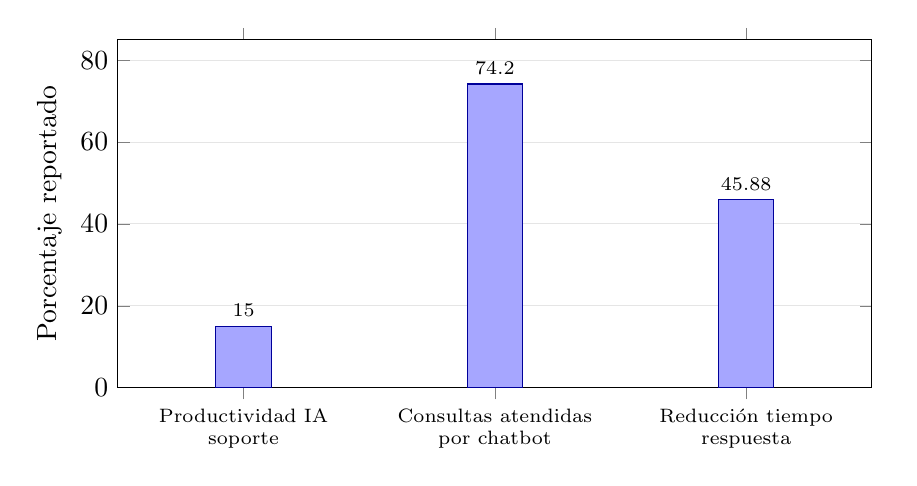
\begin{tikzpicture}
\begin{axis}[
    ybar,
    width=0.92\textwidth,
    height=6cm,
    ymin=0,
    ymax=85,
    ylabel={Porcentaje reportado},
    symbolic x coords={prod,auto,tiempo},
    xtick=data,
    xticklabels={{Productividad IA\\soporte},{Consultas atendidas\\por chatbot},{Reducción tiempo\\respuesta}},
    xticklabel style={align=center,font=\scriptsize,text width=34mm},
    ymajorgrids=true,
    grid style={gray!20},
    bar width=20pt,
    nodes near coords,
    every node near coord/.append style={font=\scriptsize},
    nodes near coords align={vertical},
    enlarge x limits=0.25
]
\addplot[fill=blue!35,draw=blue!60!black] coordinates {(prod,15) (auto,74.2) (tiempo,45.88)};
\end{axis}
\end{tikzpicture}
\caption{Evidencia externa usada para orientar métricas del piloto de DeliverAI\@. Los indicadores son heterogéneos y no deben interpretarse como una comparación directa de ROI.}%
\label{fig:evidencia_automatizacion}
\end{figure}

\begin{table}[htbp]
\centering
\caption{Lectura de estudios externos para el piloto de \mbox{DeliverAI}}%
\label{tab:evidencia_externa}
\small
\begin{tabular}{@{}>{\raggedright\arraybackslash}p{3.4cm}>{\raggedright\arraybackslash}p{5.3cm}>{\raggedright\arraybackslash}p{5.5cm}@{}}
\toprule
\textbf{Estudio} & \textbf{Hallazgo relevante} & \textbf{Relación con DeliverAI} \\ \midrule
Brynjolfsson et al.\ (2025) & IA conversacional aumentó la productividad de agentes de soporte en 15\%. & Refuerza el enfoque de asistencia conversacional con humano responsable, especialmente para reducir curva operativa. \\
Marcineková et al.\ (2025) & Chatbot en microempresa atendió 74.2\% de consultas y redujo el tiempo promedio de respuesta en 45.88\%. & Es el análogo más cercano: comercio digital, atención repetitiva, escalamiento humano y satisfacción del cliente. \\
Lacity et al.\ (2015) & Telefónica O2 mostró payback cercano a 12 meses y despliegue inicial rápido en procesos RPA seleccionados. & Sirve como benchmark ejecutivo de automatización transaccional; debe usarse con cautela por su escala empresarial. \\ \bottomrule
\end{tabular}
\end{table}

El valor esperado no debe expresarse como una cifra inventada. La hipótesis defendible es que DeliverAI puede reducir el tiempo de confirmación, aumentar la proporción de pedidos completos y mejorar la trazabilidad. Si el piloto no muestra mejora frente a la línea base o si la operación humana aumenta por fallbacks excesivos, el proyecto debe ajustarse o detenerse.
